\documentclass[11pt]{article}

\usepackage[margin=1in]{geometry}
\usepackage{amsmath,amssymb}
\usepackage{listings}
\usepackage{xcolor}
\usepackage[hidelinks]{hyperref}

\usepackage{tikz}


\lstset{
  basicstyle=\ttfamily\small,
  keywordstyle=\color{black}\bfseries,
  commentstyle=\color{gray},
  breaklines=true,
  frame=single,
  framerule=0.4pt,
  xleftmargin=1em,
  framexleftmargin=0.5em,
  columns=fullflexible,
  keepspaces=true,
  aboveskip=1em,
  belowskip=1em,
}

\definecolor{accentblue}{RGB}{30, 64, 175}

\lstset{
    basicstyle=\ttfamily\small,
    escapeinside={(*@}{@*)},
    frame=single,
    breaklines=true,
}

\newcommand{\added}[1]{\textcolor{accentblue}{#1}}

\title{Facts, Episodes, and Narratives:\\
A Canonical Internal Schema for Phoros}
\author{Marcus A. Thomas}
\date{Feb 21 2026}

\begin{document}
\maketitle

\section{Overview}

This document specifies the internal data schema for Phoros. The schema
organizes clinical data into three layers: \textbf{Facts} (atomic clinical
events), \textbf{Episodes} (problem-centric groupings of facts over time),
and \textbf{Narratives} (authored interpretations of episodes). We refer to
this as the FEN schema.

The schema is defined as Rust types. Storage is abstracted: the types do not
assume a relational database, document store, or any particular persistence
mechanism. The choice of storage backend is a separate decision, downstream
of the domain model.

Section~\ref{sec:value-types}
defines shared value types. Section~\ref{sec:traits} introduces traits and
explains where polymorphism is and is not warranted.
Section~\ref{sec:design-decisions} explains the key structural decisions and
their rationale. Section~\ref{sec:tradeoffs} addresses tradeoffs.

\subsection{Entities, Relations, and Graph Representation}

The FEN schema adopts a graph-oriented representation. Facts, problem
episodes, and narratives are nodes. Relations between them are directed,
typed edges. Every edge is an episode relation or narrative relation and
carries a \texttt{relation\_type}. Supersession is one such relation type
and is represented within this same framework.

This avoids embedding relational structure inside entity definitions.
All inter-entity structure is expressed uniformly through authored
relations with explicit assertion metadata.



\begin{center}
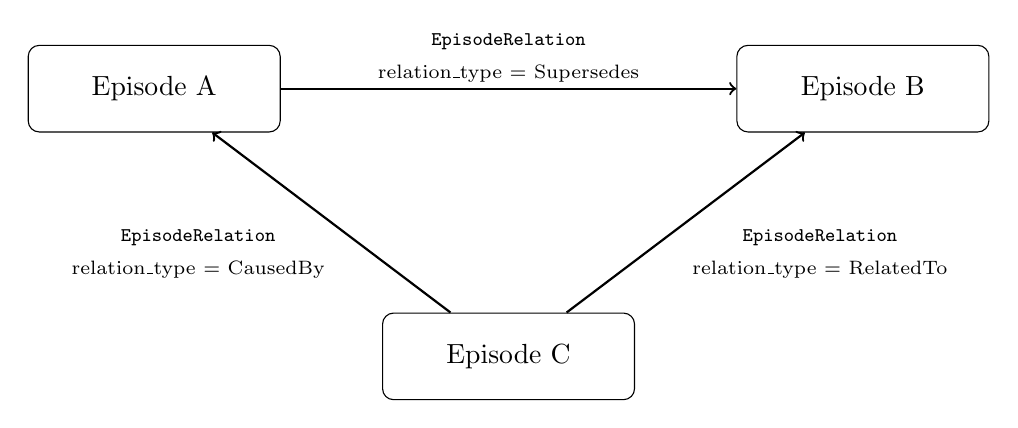
\begin{tikzpicture}[
    entity/.style={
        draw,
        rounded corners,
        minimum width=3.2cm,
        minimum height=1.1cm,
        align=center
    },
    edge/.style={->, thick},
    relation/.style={draw=none, fill=white, inner sep=2pt, align=center}
]

\node[entity] (A) at (0,0) {Episode A};
\node[entity] (B) at (9,0) {Episode B};
\node[entity] (C) at (4.5,-3.4) {Episode C};

\draw[edge] (A) -- node[relation, above]
    {\scriptsize\texttt{EpisodeRelation}\\\scriptsize relation\_type = Supersedes} (B);

\draw[edge] (C) -- node[relation, below left]
    {\scriptsize\texttt{EpisodeRelation}\\\scriptsize relation\_type = CausedBy} (A);

\draw[edge] (C) -- node[relation, below right]
    {\scriptsize\texttt{EpisodeRelation}\\\scriptsize relation\_type = RelatedTo} (B);

\end{tikzpicture}
\end{center}

\subsection{Fact}
\label{sec:entities}

A \texttt{Fact} is the atomic unit of the schema. It represents a single
clinical or scientific or administrative event grounded in evidence: a measurement, a
prescription, a procedure, a diagnosis, an imaging result, a note, an
encounter, or a billing and insurance event (coverage enrollment, claim
submission, adjudication, pre-authorization, appeal). Facts are time-indexed
and evidence-groundable. They are closer to raw observations and institutional
actions than to interpretation.

Alternately, a Fact is a dated epistemic assertion accepted
into the record. It may be observed, authored, reported, extracted, or inferred.
Its assertion metadata tells us who or what asserted it and how. Its evidence
references tell us what supports it. Its status tells us how the system presently
regards it. None of these guarantees that its content is true.

\begin{lstlisting}
Fact {
    id:              FactId,
    subject_id:      SubjectId,
    occurred_at:     TemporalAnchor,
    code:            Option<CodedValue>,
    payload:         FactPayload,
    status:          FactStatus,
    assertion:       AssertionProvenance,
    evidence:        Vec<EvidenceRef>,
    external_refs:   Vec<ExternalRef>,
}
\end{lstlisting}

This separation answers four different questions without duplicating source
metadata inside every Fact:

\begin{enumerate}
\item \texttt{SourceArtifact}: what bytes or source package did Phoros receive?
\item \texttt{ProcessingRun}: how were those bytes interpreted?
\item \texttt{EvidenceRef}: which source citation or prior Fact supports this Fact?
\item \texttt{AssertionProvenance}: who or what asserted this Fact, when, and by what method?
\end{enumerate}

\paragraph{Three concrete cases.}
\begin{itemize}
\item \textbf{Clinician-authored Fact.} The assertion method is \texttt{Authored};
  \texttt{evidence} may be empty when no separate evidentiary object is represented.
\item \textbf{Fact extracted from a PDF.} The assertion method is \texttt{Extracted};
  \texttt{evidence} contains a \texttt{SourceCitationRef} locating the relevant PDF page.
\item \textbf{Inferred Fact.} The assertion method is \texttt{Inferred};
  its evidence may combine prior-Fact references (\texttt{PriorFact}) with
  direct source citations.
\end{itemize}

In all three cases the object remains a Fact: an atomic epistemic assertion.
Episodes remain problem-centric groupings of Facts, and Narratives remain
authored interpretations. Neither is collapsed into Fact evidence.



\texttt{FactPayload} is a sum type carrying the type-specific data for each
fact variant. This replaces a generic value field with a structured enum
whose variants correspond to \texttt{FactType}. The rationale for using an
enum rather than trait objects for fact-type-specific data is discussed in
Section~\ref{sec:traits-not}.

\begin{lstlisting}
FactPayload {
    Measurement { magnitude: f64, unit: String, relevant_note: Option<FactId>  },
    Prescription { medication: CodedValue, dosage: Dosage,
                   frequency: Frequency, period: Option<TimeInterval>, relevant_note: Option<FactId> }
    Administration { medication: CodedValue, dosage: Dosage,
                     relevant_note: Option<FactId>  },
    Procedure { site: Option<CodedValue>,
                laterality: Option<Laterality>, relevant_note: Option<FactId> },
    Diagnosis { relevant_note: Option<FactId> },
    ImagingResult { modality: String, body_site: Option<CodedValue>,
                    relevant_note: Option<FactId>  },
    LabResult { value: f64, unit: String,
                reference_range: Option<ReferenceRange>, relevant_note: Option<FactId> ,
    Note { content: String, note_type: NoteType },
    Encounter { encounter_type: EncounterType,
                facility: Option<String>, relevant_note: Option<FactId>  },
    Referral { to_specialty: String, reason: String },
    Document { document_type: String, content_ref: DocumentRef },
    Coverage { payer: String, plan: String,
               member_id: String, group_id: Option<String>,
               coverage_type: CoverageType, relevant_note: Option<FactId>  },
    Claim { claim_id: String, billed_codes: Vec<CodedValue>,
            billed_amount: Money, payer: String, relevant_note: Option<FactId>  },
    Adjudication { claim_id: String, allowed_amount: Money,
                   patient_responsibility: Money,
                   status: AdjudicationStatus, relevant_note: Option<FactId>  },
    Payment { claim_id: String, amount: Money,
              paid_by: PayerType, relevant_note: Option<FactId>  },
    PreAuthRequest { requested_service: CodedValue,
                     payer: String,
                     authorization_id: Option<String>,
                     relevant_note: Option<FactId> },
    PreAuthDecision { authorization_id: String,
                      status: AuthorizationStatus,
                      reason: Option<String>,
                      approved_service: Option<CodedValue>,
                      valid_through: Option<Date>,relevant_note: Option<FactId>  },
    Appeal { original_decision_id: FactId,
             grounds: String,
             supporting_facts: Vec<FactId>, relevant_note: Option<FactId>  },
}
\end{lstlisting}

\texttt{FactStatus} tracks the correctness state of a fact:

\begin{lstlisting}
pub enum FactStatus {
    Active,
    (*@\added{Superseded \{}@*)
        (*@\added{superseded\_by: Author,}@*)
        (*@\added{superseded\_at: TemporalAnchor,}@*)
        (*@\added{replaced\_by:   Option<FactId>,}@*)
        (*@\added{reason:        SupersessionReason,}@*)
    (*@\added{\},}@*)
    EnteredInError {
        corrected_by: Author,
        corrected_at: TemporalAnchor,
        replaced_by:  Option<FactId>,
    },
}
\end{lstlisting}


A fact either happened or it did not. Facts are not versioned. If a fact is
updated or wrong, its \texttt{status} is set to \texttt{Superseded} or
\texttt{EnteredInError}, and a new fact may be created to replace it.
The \texttt{SupersessionReason} signifies a newer version of the fact exists without implying the original was wrong:
\begin{lstlisting}
pub enum SupersessionReason {
    AiEnrichment,
    ClinicalRefinement,   // e.g. a clinician updates a working diagnosis
                          // to confirmed -- not an error, just evolution
}
\end{lstlisting}

\texttt{TemporalAnchor} represents either a point in time or a period:

\begin{lstlisting}
TemporalAnchor {
    Point(Timestamp),
    Period { start: Timestamp, end: Timestamp },
}
\end{lstlisting}

\subsection{ProblemEpisode}

A \texttt{ProblemEpisode} is a persistent object representing a coherent
clinical problem, question, or management thread over time. An episode may
span multiple encounters, involve multiple care sites, and include diverse
fact types. It is not a time window. It is the assertion that a set of
clinical events belong to the same problem.

\begin{lstlisting}
ProblemEpisode {
    id:              ProblemEpisodeId,
    subject_id:      SubjectId,
    label:           String,
    problem_code:    Option<CodedValue>,
    status:          EpisodeStatus,
    onset:           Option<ApproximateDate>,
    authored_by:     Author,
    authored_at:     Timestamp,
    notes:           Option<String>,
}
\end{lstlisting}

\texttt{EpisodeStatus} captures the current clinical phase of the problem:

\begin{lstlisting}
pub struct ResolutionInfo {
    pub at: Option<ApproximateDate>,
}

pub enum EpisodeStatus {
    Active,
    Dormant,
    Resolved(ResolutionInfo),
}
\end{lstlisting}

\subsection{EpisodeMembership}

\texttt{EpisodeMembership} is the struct that links a fact to an episode. It
is a standalone entity, not a list on \texttt{ProblemEpisode}. This is a
central design decision explained in Section~\ref{sec:membership-rationale}.

\begin{lstlisting}
MembershipStatus {
    Active,
    Retracted {
        retracted_by: Author,
        retracted_at: TemporalAnchor},
}
\end{lstlisting}

\begin{lstlisting}
EpisodeMembership {
    id:              MembershipId,
    fact_id:         FactId,
    episode_id:      ProblemEpisodeId,
    role:            FactRole,

    asserted_by:     Author,
    asserted_at:     TemporalAnchor,
    status:          MembershipStatus,
}
\end{lstlisting}

\texttt{FactRole} describes the function a fact plays within an episode:

\begin{lstlisting}
FactRole {
    TriggeringSymptom,
    DiagnosticTest,
    Treatment,
    OutcomeMeasure,
    Monitoring,
    Complication,
    Referral,
    Administrative,
    InsuranceAction,
    Other,
}
\end{lstlisting}



\subsection{EpisodeRelation}

\texttt{EpisodeRelation} represents an asserted relationship between two
episodes. Problems cause other problems, complicate each other, split,
and merge. These relationships are not inferred by the system; they are
authored claims with an identified author and assertion time.

\begin{lstlisting}
EpisodeRelation {
    id:                  RelationId,
    source_episode_id:   ProblemEpisodeId,
    target_episode_id:   ProblemEpisodeId,
    relation_type:       EpisodeRelationType,
    asserted_by:         Author,
    asserted_at:         Timestamp,
}
\end{lstlisting}

\begin{lstlisting}
EpisodeRelationType {
    CausedBy,
    Complicates,
    Supersedes,
    SplitFrom,
    MergedInto,
    RelatedTo,
    PartOf,
}
\end{lstlisting}
\paragraph{Semantics of \texttt{PartOf}.}
The \texttt{PartOf} relation models structural containment between episodes. It should be used when a lower-level episode is one component of a broader higher-level episode, rather than when one episode causes, supersedes, or merely resembles another.

\begin{lstlisting}
EpisodeRelation {
    source_episode_id: lower_level_episode,
    target_episode_id: higher_level_episode,
    relation_type: PartOf,
    asserted_by: Author,
    asserted_at: Timestamp,
}
\end{lstlisting}

Thus, the direction of the relation is:

\begin{center}
\texttt{component episode} $\;\xrightarrow{\texttt{PartOf}}\;$ \texttt{aggregate episode}
\end{center}

For example, an onboarding workflow may be represented as a higher-level episode composed of several independently auditable lower-level episodes:

\begin{lstlisting}
SubjectRegistrationEpisode      PartOf InitialIdentityOnboardingEpisode
DeviceBindingEpisode            PartOf InitialIdentityOnboardingEpisode
ContinuityEnrollmentEpisode     PartOf InitialIdentityOnboardingEpisode
ProviderIdentityLinkingEpisode  PartOf InitialIdentityOnboardingEpisode
PayerIdentityLinkingEpisode     PartOf InitialIdentityOnboardingEpisode
\end{lstlisting}

This preserves separate authorship, timestamps, evidence, retries, and contestability for each component episode, while still allowing the system to present them as one coherent higher-level workflow.

The same pattern generalizes beyond onboarding:

\begin{lstlisting}
LabFollowUpEpisode              PartOf DiagnosticWorkupEpisode
PriorAuthorizationAppealEpisode PartOf InsuranceDisputeEpisode
RecoveryVerificationEpisode     PartOf AccountRecoveryEpisode
DelegationReviewEpisode         PartOf AuthoritySetupEpisode
\end{lstlisting}

\texttt{PartOf} should not be used for causal, corrective, or replacement relationships. Those remain represented by more specific relation types such as \texttt{CausedBy}, \texttt{Supersedes}, \texttt{SplitFrom}, or \texttt{MergedInto}.
\subsection{Narrative}

A \texttt{Narrative} is an authored interpretation of an episode. It is an
explanation: what happened, what it means, what was decided and why. Multiple
narratives per episode is the normal case. A patient, a primary care
physician, and a specialist may each author a narrative for the same episode.
These narratives may agree, partially overlap, or contradict each other.

\begin{lstlisting}
Narrative {
    id:              NarrativeId,
    episode_id:      ProblemEpisodeId,
    author:          Author,
    authored_at:     Timestamp,
    status:          NarrativeStatus,
    summary:         String,
    sections:        Vec<NarrativeSection>,
    decision_points: Vec<DecisionPoint>,
}
\end{lstlisting}

\begin{lstlisting}
NarrativeStatus {
    Draft,
    Current,
    Superseded,
}
\end{lstlisting}



\subsection{NarrativeRelation}

\begin{lstlisting}
NarrativeSupersessionInfo {
    pub note: Option<String>,
}
\end{lstlisting}

\begin{lstlisting}
ContestationInfo {
    pub scope: Option<ContestationScope>,
    pub rationale: Option<String>,
    pub effective_at: Option<TemporalAnchor>,
}
\end{lstlisting}
\begin{lstlisting}
ContestationScope {
    Partial,
    Full,
}
\end{lstlisting}

\begin{lstlisting}
NarrativeRelationType {
    Supersedes(NarrativeSupersessionInfo),
    Contests(ContestationInfo),
    RelatedTo,
}
\end{lstlisting}
\begin{lstlisting}
NarrativeRelation {
    id:                   RelationId,
    source_narrative_id:  NarrativeId,
    target_narrative_id:  NarrativeId,
    relation_type:        NarrativeRelationType,
    asserted_by:          Author,
    asserted_at:          TemporalAnchor,
}
\end{lstlisting}
\subsection{NarrativeSection}

\texttt{NarrativeSection} provides optional internal structure within a
narrative. Not all narratives require sections; the \texttt{summary} field
on \texttt{Narrative} may suffice for simple episodes. Sections are useful
when a narrative needs to distinguish phases of a problem or reference
specific facts within a larger explanation.

\begin{lstlisting}
NarrativeSection {
    id:               SectionId,
    narrative_id:     NarrativeId,
    section_type:     SectionType,
    content:          String,
    referenced_facts: Vec<FactId>,
}
\end{lstlisting}

\begin{lstlisting}
SectionType {
    Onset,
    Workup,
    Diagnosis,
    Treatment,
    Response,
    Progression,
    Resolution,
    OpenQuestions,
}
\end{lstlisting}

\subsection{DecisionPoint}

A \texttt{DecisionPoint} is a structured record of a clinical decision: what
triggered it, what action was taken, and why. It is nested within
\texttt{Narrative}, not a standalone top-level entity. The rationale for this
nesting is discussed in Section~\ref{sec:decision-point-rationale}.

\begin{lstlisting}
DecisionPoint {
    id:               DecisionPointId,
    narrative_id:     NarrativeId,
    occurred_at:      Timestamp,
    triggering_facts: Vec<FactId>,
    action:           DecisionAction,
    rationale:        String,
    alternatives:     Vec<Alternative>,
    author:           Author,
    authored_at:      Timestamp,
}
\end{lstlisting}

\texttt{DecisionAction} is either a reference to a fact (the prescription
that was written, the procedure that was performed) or a free-text
description when no corresponding fact exists (e.g., a decision to defer
action):

\begin{lstlisting}
DecisionAction {
    FactReference(FactId),
    Description(String),
}
\end{lstlisting}

\subsection{Alternative}

An \texttt{Alternative} is an option considered but not taken. It is nested
inside a \texttt{DecisionPoint}.

\begin{lstlisting}
Alternative {
    description:       String,
    reason_not_taken:  String,
}
\end{lstlisting}

\section{Shared Value Types}
\label{sec:value-types}

\subsection{Assertion provenance and evidence}

\texttt{AssertionProvenance} describes the act by which a Fact entered the
epistemic record. It does not repeat source receipt, document, or import
metadata.

Assertion provenance and evidence are orthogonal. The former describes the
act of making or accepting a claim; the latter describes the basis for that
claim. Different assertions may cite the same evidence, and one assertion may
depend on several pieces of evidence.

\begin{lstlisting}
AssertionProvenance {
    asserted_by:      Author,
    asserted_at:      Timestamp,
    method:           AssertionMethod,
}

AssertionMethod {
    Observed,
    Reported,
    Authored,
    Extracted,
    Inferred,
}

EvidenceRef {
    Source(SourceCitationRef),
    PriorFact(FactId),
}
\end{lstlisting}

\texttt{SourceCitationRef} is a typed foreign reference to the source-artifact
domain. That domain owns the received bytes, receipt provenance, processing
run, and format-aware location. The FEN schema owns only the reference.

\texttt{PriorFact} supports derived assertions without treating Episodes or
Narratives as raw evidence. Fact-to-Fact evidence links must be acyclic: a Fact
cannot support itself, directly or transitively.

\subsubsection{Canonical references and downstream exports}

The canonical FEN representation keeps typed evidence references rather than
copying source metadata into every Fact. A self-contained downstream export
may resolve those references into a materialized provenance envelope. That
envelope is an export projection, not a second canonical provenance model.

The separate \texttt{FactOperational} representation remains warranted for
indexing, policy evaluation, and encrypted-payload location. It should carry
only the assertion or evidence identifiers and summaries required by those
operational uses, rather than duplicating full source provenance.

\subsection{Author}

\begin{lstlisting}
Author {
    author_type:  AuthorType,
    author_id:    Option<AuthorId>,
    display_name: Option<String>,
}
\end{lstlisting}

\begin{lstlisting}
AuthorType {
    Patient,
    Clinician,
    System,
    AiAssisted,
}
\end{lstlisting}

\subsection{CodedValue}

\begin{lstlisting}
CodedValue {
    system:   CodingSystem,
    code:     String,
    display:  String,
}
\end{lstlisting}

\begin{lstlisting}
CodingSystem {
    SNOMED,
    ICD10,
    LOINC,
    RxNorm,
    CPT,
    Local,
}
\end{lstlisting}

\subsection{ApproximateDate}

\begin{lstlisting}
ApproximateDate {
    date:       Date,
    precision:  DatePrecision,
}
\end{lstlisting}

\begin{lstlisting}
DatePrecision {
    Day,
    Month,
    Year,
    Approximate,
}
\end{lstlisting}

\subsection{ExternalRef}

\begin{lstlisting}
ExternalRef {
    system:         ExternalSystem,
    resource_type:  Option<String>,
    resource_id:    String,
    uri:            Option<String>,
}
\end{lstlisting}

\begin{lstlisting}
ExternalSystem {
    FHIR,
    OMOP,
    CCDA,
    Other,
}
\end{lstlisting}

\texttt{ExternalRef} identifies a corresponding record in an outside
standard or system. It is not evidentiary grounding; evidentiary support is
represented by \texttt{EvidenceRef}.

\subsection{Billing and insurance value types}

\begin{lstlisting}
Money {
    amount:   f64,
    currency: String,
}
\end{lstlisting}

\begin{lstlisting}
CoverageType {
    Commercial,
    Medicare,
    Medicaid,
    Tricare,
    SelfPay,
    Other,
}
\end{lstlisting}

\begin{lstlisting}
AdjudicationStatus {
    Paid,
    Denied,
    PartiallyPaid,
    Pending,
}
\end{lstlisting}

\begin{lstlisting}
PayerType {
    PrimaryInsurance,
    SecondaryInsurance,
    Patient,
    Other,
}
\end{lstlisting}

\begin{lstlisting}
AuthorizationStatus {
    Approved,
    Denied,
    PartiallyApproved,
    Pending,
    Appealed,
}
\end{lstlisting}

\section{Traits}
\label{sec:traits}

The schema uses traits selectively. Traits capture shared \emph{behavior}
that the system needs to dispatch on polymorphically. They are not used
merely because two structs share field names. This section identifies two
traits that are warranted by concrete system requirements and one case where
a trait-based design would be wrong.

\subsection{Temporal}
\label{sec:trait-temporal}

The system must place heterogeneous objects on a single timeline. Facts have
\texttt{occurred\_at}. Decision points have \texttt{occurred\_at}. Episode
status changes and narrative revisions have timestamps. A timeline view
that interleaves these objects needs a common interface for temporal
position.

\begin{lstlisting}
trait Temporal {
    fn temporal_anchor(&self) -> TemporalAnchor;
}
\end{lstlisting}

With this trait, the system can collect \texttt{Vec<\&dyn Temporal>} from
heterogeneous entity types and sort or render them on a unified timeline
without matching on every concrete type. \texttt{Fact}, \texttt{DecisionPoint},
\texttt{EpisodeMembership} (via \texttt{asserted\_at}), and
\texttt{Narrative} (via \texttt{authored\_at}) all implement this trait.

The alternative---matching on an enum of all possible timeline
entries---works when the set of temporal entities is small and closed. But as
the schema grows, the enum becomes a maintenance burden. The trait keeps
timeline logic decoupled from the entity definitions.

\subsection{Authored}
\label{sec:trait-authored}

\texttt{Fact} carries authorship through \texttt{AssertionProvenance}.
Authorship also appears on membership and relation claims, Narratives, and
DecisionPoints. If the system needs to answer ``show me
everything authored or asserted by Dr.~X,'' a trait provides a uniform
interface across entity types.

\begin{lstlisting}
trait Authored {
    fn author(&self) -> &Author;
    fn authored_at(&self) -> Timestamp;
}
\end{lstlisting}

This trait is warranted only if cross-entity authorship queries are a real
use case. If the system never collects heterogeneous entities into a single
author-filtered view, the trait adds ceremony without purpose. The
current expectation is that authorship queries \emph{are} a core
requirement: audit logs, author-filtered views, and consent scoping all
require answering ``who asserted what, and when'' across entity boundaries.


\subsection{Where traits are not the right tool}
\label{sec:traits-not}

\paragraph{Fact types.}
The \texttt{FactType} enum is a closed set controlled by Phoros. One might
be tempted to model \texttt{Fact} as a trait with separate structs for
\texttt{Measurement}, \texttt{Prescription}, \texttt{Procedure}, and so on,
each carrying type-specific fields. This is the wrong approach in Rust.

A closed set of variants is an enum, not a trait hierarchy. Enums provide
exhaustive pattern matching: the compiler enforces that every handler covers
every variant. They require no heap allocation. They allow value semantics.
Trait objects lose all three properties.

The correct design is \texttt{FactPayload}, defined in
Section~\ref{sec:entities}: a sum type whose variants carry the
type-specific data for each fact kind. \texttt{Fact} holds the common fields
(\texttt{id}, \texttt{subject\_id}, \texttt{occurred\_at},
\texttt{assertion}, \texttt{evidence}, etc.) and a \texttt{FactPayload} for the variant data.
Adding a new fact type means adding a variant to the enum. The compiler will
then identify every \texttt{match} expression that needs to handle the new
variant.

If \texttt{FactType} were an open set---if external systems could register
new fact types at runtime---trait objects would be justified. That is not the
current design.

\paragraph{Shared fields without shared behavior.}
\texttt{EpisodeMembership} and \texttt{EpisodeRelation} both have
\texttt{asserted\_by: Author} and \texttt{asserted\_at: Timestamp}. This
structural overlap does not, by itself, justify a trait. A trait is warranted
only when the system dispatches generically over the shared interface. If
these two types are never collected into the same container and never passed
to the same generic function, repeating the fields is clearer than
introducing an abstraction with no consumer.

The \texttt{Authored} trait covers this case only if cross-entity authorship
queries materialize as a requirement. If they do not, the shared fields
remain coincidental, and the trait should not exist.

\subsection{Summary of trait usage}

\begin{center}
\renewcommand{\arraystretch}{1.3}
\begin{tabular}{l l l}
\textbf{Pattern} & \textbf{Mechanism} & \textbf{Reason} \\
\hline
Timeline placement & \texttt{Temporal} trait &
  Heterogeneous collection, single sort \\
Authorship queries & \texttt{Authored} trait &
  Generic ``who authored this'' across types \\
Fact-type-specific data & \texttt{FactPayload} enum &
  Closed set, exhaustive matching \\
Shared fields only & Repeat the fields &
  No behavioral need for abstraction \\
\end{tabular}
\end{center}

The guiding principle is: use traits when the system needs to \emph{do the
same thing} to different types. Use enums when the system needs to
\emph{distinguish} between a fixed set of variants. Repeat fields when
structural similarity does not correspond to behavioral polymorphism.

\section{Design Decisions}
\label{sec:design-decisions}

\subsection{Why EpisodeMembership is a standalone struct}
\label{sec:membership-rationale}

A \texttt{ProblemEpisode} does not contain a \texttt{Vec<FactId>}. Instead,
\texttt{EpisodeMembership} is a standalone struct that references both a
\texttt{FactId} and a \texttt{ProblemEpisodeId}. The episode is defined by the
set of memberships that point to it, not by an internal collection it owns.

This design has four advantages.

\paragraph{Granular contestability.}
Assigning a fact to an episode is itself a claim, and claims need explicit
authorship and assertion time.
A patient may assert that a lab result belongs to their chronic kidney disease
episode. A nephrologist may assert the same lab result belongs to an acute
injury episode. Both memberships exist simultaneously with different authors.
Neither the episode nor the fact needs to be duplicated. The disagreement
lives where it should: in the membership records.

\paragraph{Multi-episode membership.}
A single fact can belong to multiple episodes without ambiguity. A potassium
level may be relevant to both a cardiac arrhythmia episode and a CKD episode.
Two memberships, two roles, possibly two different authors. A
\texttt{Vec<FactId>} on the episode can express multiplicity, but it cannot
express \emph{why} or \emph{who said so} for each assignment.

\paragraph{Audit and revision.}
The question ``when was this fact added to this episode, and by whom?'' is
answered directly by the membership record. If an episode is reorganized---a
fact is reassigned from one episode to another---the old membership is
retained or marked superseded, and a new one is created. The history of the
grouping is preserved.

\paragraph{Role annotation.}
The \texttt{role} field on membership records the function a fact plays
within an episode. The same fact may serve as a diagnostic test in one
episode and as a monitoring measure in another. This structure does not exist
on a flat list.


\subsection{Why EpisodeRelation is explicit}
\label{sec:relation-rationale}

The system does not infer that diabetes caused chronic kidney disease. If
that relationship is part of the record, someone asserted it. The
\texttt{EpisodeRelation} struct records who, when, and what type of
relationship is claimed.

This is a constraint. It means the system will not automatically link
related problems. The benefit is that every inter-episode link has explicit
assertion metadata
and can be audited, contested, or removed. The alternative---inferring
relationships from co-occurrence, shared codes, or temporal
proximity---produces links that no one authored and no one can explain.

\subsection{Why DecisionPoint is nested under Narrative}
\label{sec:decision-point-rationale}

A \texttt{DecisionPoint} is not a standalone top-level entity. It is a
component of \texttt{Narrative}. It inherits the authorship and assertion context
of its parent narrative.

The rationale: a decision rationale is not a fact. It is an explanation of
why certain facts led to certain actions. That is narrative. Promoting it to
a standalone entity would add a fourth top-level layer (Facts, Episodes,
Decisions, Narratives) and raise the question of where decisions sit relative
to narratives. Since a well-structured narrative already contains decision
rationale, the nesting avoids redundancy.

There is one condition under which promotion is warranted. If decision
rationale needs to be \emph{independently contestable}---for instance, a
patient disputes the stated reason for a medication change, or a second
opinion challenges the reasoning behind a surgical decision---then the
\texttt{DecisionPoint} may need its own identity and versioning separate
from the narrative that contains it. The recommendation is to start nested
and promote if this requirement materializes in practice.

\subsection{Why billing and insurance are Facts}
\label{sec:billing-rationale}

The schema represents billing events (claims, adjudications, payments),
insurance coverage, pre-authorization requests and decisions, and appeals as
\texttt{Fact} variants rather than as a separate billing domain.

The rationale is twofold. First, these are events. A patient enrolled in a
plan at a specific time. A claim was submitted on a specific date. A
pre-authorization was denied with a stated reason. Each has a timestamp,
assertion provenance, and whatever evidence is available. They satisfy the
definition of a Fact.

Second, billing events are clinically relevant. A denied pre-authorization
for an MRI belongs to the same \texttt{ProblemEpisode} as the back pain that
prompted it. A claim adjudication that reduces a billed amount is part of the
patient's experience of managing that problem. Excluding billing from the
Fact layer would force the most financially consequential information outside
the representational model that supports patient understanding.

Coverage is a Fact because enrollment is an action the patient took at a
specific time. The coverage period is a consequence of that action, captured
by \texttt{TemporalAnchor::Period}. This is analogous to a prescription: an
action at time $t$ that produces an effect over a period $[t_1, t_2]$.

Not all billing Facts require episode assignment. A coverage Fact is not
``about'' any particular problem. It exists in the record without
\texttt{EpisodeMembership} records pointing to it. The schema permits this:
\texttt{EpisodeMembership} is a separate struct, so unassigned Facts are
simply Facts with no membership records. Claims, pre-authorizations, and
appeals, by contrast, are typically episode-specific and should be assigned
via \texttt{EpisodeMembership} with role \texttt{InsuranceAction}.

\section{Tradeoffs}
\label{sec:tradeoffs}

\subsection{Indirection cost of EpisodeMembership}

Resolving ``all facts in this episode'' requires traversing
\texttt{EpisodeMembership} records rather than reading a
\texttt{Vec<FactId>} from the episode struct. This is an indirection cost.
The magnitude of the cost depends on the storage backend, which the schema
does not prescribe.

For read-heavy product surfaces, a denormalized view---episode with its
resolved facts---can be materialized and cached. The source of truth remains
the membership records, because that is where the grouping assertion and its
authorship live. The
denormalized view is a performance optimization, not the data model.




\section{Relationship to FHIR and existing standards}

FHIR provides \texttt{EpisodeOfCare} and \texttt{Condition} resources that
partially overlap with the episode concept described here. However,
\texttt{EpisodeOfCare} is scoped to a single managing organization and care
period; it is an administrative rather than clinical grouping.
\texttt{Condition} represents a clinical assertion but does not structurally
contain the heterogeneous facts (labs, medications, procedures, notes)
associated with managing that condition over time. ICD/SNOMED problem lists
enumerate active conditions but do not represent temporal evolution, phase
transitions, or interpretive disagreement. The \texttt{ProblemEpisode} entity
proposed here fills a specific gap: a persistent, cross-encounter, multi-fact
grouping that is authorable, and contestable. It is not a
replacement for these standards but a layer that organizes what they provide.

The schema maintains interoperability through two mechanisms. First,
\texttt{ExternalRef} on \texttt{Fact} preserves references to FHIR resource
URIs, OMOP concept IDs, and C-CDA document identifiers. Second,
\texttt{CodedValue} uses standard terminologies (SNOMED, ICD-10, LOINC,
RxNorm, CPT). The FEN schema does not replace external standards. It ingests
from them and can export to them. The layering is:
\[
\begin{aligned}
\text{Ingest external standards} &\;\rightarrow\; \text{normalize as Facts} \\
&\;\rightarrow\; \text{lift into Episodes}
  \;\rightarrow\; \text{host Narratives as interpretations.}
\end{aligned}
\]


\section{Summary}
\enlargethispage{\baselineskip}

The FEN schema defines nine entity types organized in three layers, with
two traits that provide cross-cutting behavior:

\begin{center}
\footnotesize
\renewcommand{\arraystretch}{1.15}
\begin{tabular}{l l l}
\textbf{Layer} & \textbf{Entities} & \textbf{Ontological status} \\
\hline
Facts      & \texttt{Fact}
           & Observations and actions \\
Episodes   & \texttt{ProblemEpisode}, \texttt{EpisodeMembership}, \texttt{EpisodeRelation}
           & Structured hypotheses \\
Narratives & \texttt{Narrative}, \texttt{NarrativeSection}, \texttt{DecisionPoint}, \texttt{Alternative}
           & Authored interpretations \\
\end{tabular}

\medskip

\begin{tabular}{l l}
\textbf{Trait} & \textbf{Purpose} \\
\hline
\texttt{Temporal}    & Unified timeline placement across entity types \\
\texttt{Authored}    & Cross-entity authorship queries \\
\end{tabular}
\end{center}

{\small Episodes and Narratives are first-class, contestable objects---not
derived groupings or unstructured annotations. Fact-to-Episode assignment is
therefore an assertion-bearing record, not a list. Traits support cross-type
behavior; enums ensure exhaustive matching over closed variants. This design
favors contestability, auditability, and fidelity to clinical reasoning while
accepting added indirection and storage. The Rust schema remains
storage-independent.}

\end{document}
